% Document Class =========================================================
  %\documentclass[final,3p,times]{elsarticle}   % one column
  \documentclass[final,5p,times]{elsarticle}    % two column
  % Use the options 1p,two-column; 3p; 3p,two-column; 5p; or 5p,two-column
    % for a journal layout: Use the option review to obtain double
    % line spacing
% Preamble ===============================================================
  %=================================== Document ==================================

%\usepackage[top=2.5cm, bottom=2cm, right=2cm, left=2.5cm]{geometry}
%\usepackage[portuges, brazilian]{babel} % hibernation Portuguese
\usepackage[utf8]{inputenc}             % Accentuation
%\usepackage[T1]{fontenc}
%\usepackage{setspace}                   % Change line space 
%  \onehalfspacing %\singlespacing  %\doublespacing
%\usepackage{indentfirst}                % indent first line
\usepackage{lineno,hyperref}            % Hipper-link
\hypersetup{colorlinks=true,            % Delete Box ref
  breaklinks=true, pdfauthor={Name}}    % breaking  links
\usepackage{xcolor}                     % Color Hyperref
\usepackage{etoolbox}                   % broke lines in bibliography
\hbadness 10000
\tolerance 10000
% \usepackage{lipsum}                     % Bibliography style
\usepackage{framed}                     % Box for Nomenclature
%\usepackage{titlesec}                   % change tittle configurations 
%  \titleformat
%    {\chapter}{\normalfont\LARGE \selectfont \bfseries}  % Format
%    {\thechapter}{1ex plus 1ex}{}
%  \titlespacing*
%    {\chapter}                          % command
%    {0pt}                               % left
%    {0.5\baselineskip}                  % before
%    {0.5\baselineskip}                  % after
%  \setcounter{tocdepth}{3}              % deep and subsections
%  \setcounter{secnumdepth}{3}           % sections numerations
%  \usepackage{emptypage}                  % empty page number

%================================== Equations ===================================

\usepackage{amsmath}
%\usepackage{algorithm}
%\usepackage{algorithm2e}
\usepackage{algpseudocode}
\usepackage[linesnumbered, ruled, vlined, onelanguage]{algorithm2e}
\usepackage{amssymb}

%==================================== Tables ====================================

\usepackage{booktabs}
\usepackage{tabularx}
\usepackage{pbox}                      % Pbox for tables
%\usepackage{array}
\usepackage{multirow}                   % multi rows
\usepackage{multicol}                   % multi columns
\usepackage[justification=centering]{caption} % Centering table caption
\usepackage{threeparttable}

%==================================== Images ====================================

\usepackage{graphicx}                   % cut images
\usepackage{float}                      % Make the images float
\usepackage{caption}                    % Sub-Plots
\usepackage{subcaption}                 % Sub-Plots
\usepackage{transparent}
%\usepackage{pdflscape}          % Rotate Figure

\usepackage{pgf}

%============================== Literature review ===============================

%\usepackage{cite}
%\usepackage{pdfpages}                   % Insert pdf pages

%========================= Elsevier bibliography styles =========================

%\modulolinenumbers[5]
%\bibliographystyle{styles/model1-num-names}   % Numbered
%\bibliographystyle{styles/model1a-num-names}  % Numbered without titles
%\bibliographystyle{styles/model2-names.bst}\biboptions{authoryear}  % Harvard
%----------------------  Vancouver numbered and name/year -----------------------
%\usepackage{numcompress}\bibliographystyle{styles/model3-num-names}  %  numbered
%\usepackage{numcompress}\bibliographystyle{styles/model4-names}\biboptions{authoryear} 
%-------------------------------------------------------------------------------
%\bibliographystyle{styles/model5-names}\biboptions{authoryear}      % APA style
%\usepackage{numcompress}\bibliographystyle{styles/model6-num-names} % AMA style
\bibliographystyle{styles/elsarticle-num-names}     % `Elsevier LaTeX' style
\biboptions{numbers,sort&compress}
  \journal{~}

\begin{document}

  \hypersetup{citecolor=teal, linkcolor=blue, urlcolor=gray, breaklinks=true}
  %\linenumbers

  \begin{frontmatter}

    \title{Corrosion-rate prediction strategy based on interpretable
      decision trees and fuzzy inference for reduced and imbalanced
      field databases}

    % Authors intentionally left blank.
    \author[1]{Mauricio Barrios Castellanos}
    \ead{mauricio.bc.89@gmail.com}

    \author[1]{Maria Camila Granados-Giraldo}
    \ead{mgranados@corrosioncic.com}

    \author[1]{Jhon Padilla}
    \ead{jpadilla@corrosioncic.com}

    \author[1]{Daniel Felipe Bernal-mejia}
    \ead{jpadilla@corrosioncic.com}

    \author[1]{Genis Andrés Castillo-Villamizar}
    \ead{jpadilla@corrosioncic.com}


    \address[1]{Corporación para la Investigación de la Corroción (CIC)}

    \begin{abstract}
      The prediction of the corrosion rate in industrial assets relies on
imbalanced databases, in which the observations concentrate at low
values of the target variable while the regimes of higher severity
remain under-represented, and on databases with a reduced number of
useful records. Conventional regression models underestimate the
critical conditions and compromise integrity decisions. This research
proposes a hybrid strategy that articulates segmentation by normative
ranges, interpretable classification, and fuzzy inference, with the
purpose of obtaining a reliable and auditable numerical estimator from
the knowledge extracted from the data and from expert judgment. The
methodology transforms the target variable into the classes defined by
the technical standard: 0--2 [mpy], 2--8 [mpy], and above 8 [mpy]. One
binomial decision tree per normative limit is trained under stratified
nested cross-validation, adjusting the hyperparameters with the
criterion of exceeding a mean per-class recall of 0.6. A record-level
leakage audit precedes the modeling: it revealed that a calculated
thickness-loss column reproduced the reported target exactly for
76.5\% of the records and excluded it together with its ingredients.
On the audited internal-corrosion dataset of 897 records, the trees
reached out-of-fold mean recalls of 0.71 and 0.81 at the 2 [mpy] and
8 [mpy] limits with balanced per-class sensitivity. The rule
extraction produced twelve interpretable propositions, consistent with
the service history and the operating conditions of the asset. Each
numerical partition translates into an interval membership function
anchored at the tree thresholds, and each branch reformulates as a
fuzzy rule whose consequent remains bounded to its normative range.
The fuzzy system converts these discrete rules into a continuous
output, smoothing the transitions between ranges: it reached an
out-of-fold coefficient of determination of 0.50 and a mean absolute
error of 3.6 [mpy], against 0.49 and 4.1 [mpy] for linear regression
on identical folds, with a lower error in every severity zone. The
traceability between each prediction, the active rule, and the
integrity meaning of its conditions supports expert audit of the
complete inference chain in scenarios of imbalanced and reduced data,
frequent in asset-integrity applications.

    \end{abstract}

    \begin{keyword}
      Corrosion rate \sep
      Decision trees \sep
      Fuzzy inference \sep
      Interpretable machine learning \sep
      Asset integrity.
    \end{keyword}

  \end{frontmatter}

  \section{Introduction} %================================================
    Internal corrosion governs the residual life of production piping in
mature oil fields. Integrity programs quantify its progression through
the corrosion rate $v$, expressed in mils per year [mpy], and classify
the severity against normative limits: rates up to 2 [mpy] permit
routine monitoring, rates between 2 [mpy] and 8 [mpy] require
intensified inspection, and rates above 8 [mpy] demand intervention.
Field measurement campaigns produce databases with two structural
difficulties. First, the observations concentrate in the low-severity
range, so the critical regimes remain under-represented
\cite{he2009imbalanced}. Second, the number of useful records rarely
exceeds a few hundred after quality control.

Regression models trained on such data minimize a global error and,
consequently, underestimate the scarce high-severity observations. The
resulting predictions bias inspection planning toward the benign
regimes. Flexible ensemble regressors reduce the global error
\cite{breiman2001random} but hide the reasoning behind each
prediction, which conflicts with the audit requirements of integrity
management \cite{rudin2019stop}; on reduced databases their high
parameter count also raises the risk of overfitting.

Fuzzy inference systems offer the language that integrity engineers
already use: severity classes, gradual transitions, and IF--THEN rules
\cite{zadeh1965fuzzy,mamdani1975experiment}. Their practical
difficulty lies in the construction of the rulebase and of the
membership functions, which traditionally depend on manual
elicitation \cite{guillaume2001designing}. Decision trees resolve this
difficulty: a tree trained on the normative classes yields an explicit
partition of the input space whose branches read as rules
\cite{breiman1984cart}.

This study articulates both elements into a single strategy. Binomial
decision trees, one per normative limit, provide the classification
backbone; the tree thresholds define interval membership functions
whose transition widths follow the training-data distribution; and the
resulting rulebase feeds a fuzzy inference system whose consequents
remain bounded to the normative ranges. A nested cross-validation
protocol confines every selection step to inner folds and eliminates
the optimistic bias of tune-and-refit procedures
\cite{varma2006bias,cawley2010overfitting}.

The contributions are: (i) a reproducible procedure that converts
threshold-wise decision trees into an auditable fuzzy estimator of the
corrosion rate; (ii) a distribution-based construction of interval
membership functions with transitions anchored at the tree thresholds;
(iii) a record-level leakage audit and an evaluation protocol that
together guarantee leakage-free estimates of generalization for the
complete chain; and (iv) a comparison on identical folds against
regression methods suited to reduced databases, including the
sensitivity to the severe class that drives integrity decisions.

  \section{Field data and normative segmentation} \label{sec:data} %======
    \subsection{Dataset and variables}

The study uses an internal corrosion database from a producing oil field: 903 raw records of measured corrosion rates, along with the operating conditions, produced-water chemistry, production rates, and service time for each monitoring point. Data preparation removed six records with physically invalid negative rates and the columns identified by the leakage audit of Section~\ref{sec:vmod}, leaving 897 records and 31 candidate variables. Missing entries received the training-fold median inside each cross-validation fold.

Table~\ref{tab:features} describes every variable considered with its physical meaning and unit. The set covers the CO$_2$-corrosion driving forces ($p_{\mathrm{CO_2}}$, $y_{\mathrm{CO_2}}$, $T$, $P$, pH), the water chemistry that controls scaling and conductivity ($[\mathrm{HCO_3^-}]$, $[\mathrm{Ca^{2+}}]$, $[\mathrm{Cl^-}]$, $\sigma$, TDS, Alk), the hydrodynamic and production variables that control wall shear and phase wetting ($u$, $Q_w$, $Q_o$, $Q_g$, FP), the solids content associated with under-deposit attack (TSS), and the service time $t_s$, which is fixed at installation and therefore known before any inspection.

\begin{table}[htb!]
\centering
\footnotesize
%\setlength{\tabcolsep}{2pt}
\caption{Variables of the dataset: physical meaning, units and descriptive statistics (897 records; the measured rate $v$ is reported after saturation at 20 [mpy]).}
\label{tab:features}
\begin{tabularx}{0.45\textwidth}{@{}lX@{}}
\toprule
Symbol & Meaning [unit]\\%& Min & Median & Mean & Max & Missing \\
\midrule
\midrule
$v$ & measured corrosion rate [mpy] \\%& 0 & 5.26 & 8.38 & 20 & 0 \\
$t_s$ & service time of the monitoring point [yr] \\%& -0.0219 & 9.83 & 11.8 & 38.1 & 0 \\
$p_{\mathrm{CO_2}}$ & CO$_2$ partial pressure [psig] \\%& 0 & 12 & 17.2 & 103 & 13 \\
$y_{\mathrm{CO_2}}$ & CO$_2$ gas mole fraction [--] \\%& 0 & 16 & 22.7 & 52.5 & 13 \\
$y_{\mathrm{CH_4}}$ & methane gas mole fraction [--] \\%& 0 & 46.7 & 45.6 & 87.7 & 15 \\
$y_{\mathrm{N_2}}$ & nitrogen gas mole fraction [--] \\%& -6.32 & 13.2 & 17 & 78.4 & 15 \\
$u$ & production fluid velocity [ft/s] \\%& 0 & 4.57 & 5.29 & 32.5 & 31 \\
$P$ & operating pressure [psig] \\%& 0 & 66 & 72.2 & 231 & 0 \\
$T$ & operating temperature [$^{\circ}$F] \\%& 0 & 248 & 233 & 250 & 0 \\
pH & produced-water pH [--] \\%& 0.23 & 6.85 & 6.93 & 7.88 & 14 \\
$\sigma$ & water electrical conductivity [$\mu$S/cm] \\%& -325 & 529 & 603 & 5.78e+03 & 13 \\
$[\mathrm{Cl^-}]$ & chloride concentration [ppm] \\%& -19 & 9.96 & 30.7 & 752 & 14 \\
$[\mathrm{Na^+}]$ & sodium concentration [ppm] \\%& -28.3 & 68.7 & 79.5 & 302 & 15 \\
$[\mathrm{Ca^{2+}}]$ & calcium concentration [ppm] \\%& 0.072 & 11.6 & 16.2 & 117 & 14 \\
$[\mathrm{Mg^{2+}}]$ & magnesium concentration [ppm] \\%& 0 & 4.9 & 4.54 & 12.3 & 14 \\
$[\mathrm{Ba^{2+}}]$ & barium concentration [ppm] \\%& 0 & 0.23 & 0.415 & 5.27 & 14 \\
$[\mathrm{Sr^{2+}}]$ & strontium concentration [ppm] \\%& 0 & 0.227 & 4.88 & 752 & 14 \\
$[\mathrm{Fe}]$ & total dissolved iron [ppm] \\%& -8.1 & 0.984 & 2.87 & 17.4 & 14 \\
$[\mathrm{SO_4^{2-}}]$ & sulfate concentration [ppm] \\%& -2.73 & 7.41 & 25.9 & 496 & 14 \\
$[\mathrm{HCO_3^-}]$ & bicarbonate concentration [meq/L] \\%& 1.96 & 4 & 110 & 361 & 14 \\
Alk & total alkalinity [ppm CaCO$_3$] \\%& -4 & 219 & 207 & 580 & 14 \\
TH & total hardness [ppm CaCO$_3$] \\%& 0 & 27.8 & 43.3 & 291 & 14 \\
TSS & total suspended solids [ppm] \\%& -123 & 64 & 76.2 & 437 & 14 \\
TDS & total dissolved solids [ppm] \\%& 248 & 347 & 385 & 2.03e+03 & 14 \\
$Q_w$ & water production rate [BWPD] \\%& 0 & 6.33e+03 & 8.48e+03 & 7.79e+04 & 0 \\
$Q_o$ & oil production rate [BOPD] \\%& 0 & 68.2 & 89.2 & 981 & 0 \\
$Q_g$ & gas production rate [MMSCFD] \\%& 0 & 3.29e-09 & 786 & 2.95e+04 & 0 \\
FP & flow-pattern class [--] \\%& 0 & 2 & 1.76 & 3 & 13 \\
$D$ & nominal pipe diameter [in] \\%& 3 & 4 & 4.43 & 18 & 0 \\
$D_i$ & internal pipe diameter [in] \\%& 2.07 & 3.07 & 3.16 & 17.2 & 43 \\
$D_e$ & external pipe diameter [in] \\%& 2 & 4.5 & 4.68 & 18 & 0 \\
$e$ & wall thickness [mm] \\%& 2.87 & 5.49 & 5.75 & 9.53 & 0 \\
\bottomrule
\end{tabularx}
\end{table}


\subsection{Leakage audit and excluded variables}
\label{sec:vmod}

The raw database carries a column of calculated corrosion rate, obtained from the inspection record of each monitoring point as the average thickness-loss rate over the service life,
\begin{equation}
  v_{\mathrm{calc}} = \frac{(e - e_{\min})}{t_s}
                      \cdot \frac{1000}{25.4},
  \label{eq:vmod}
\end{equation}
where $e$ [mm] is the reference wall thickness, $e_{\min}$ [mm] the minimum wall thickness measured at the point, $t_s$ [yr] the service time, and the factor $1000/25.4$ converts [mm/yr] to [mpy].  

The study consequently excludes from the candidate variables: the minimum thickness $e_{\min}$, which requires the same inspection that defines the target; the wear and remaining-life columns derived from them; and the failure flag, which labels the record itself as a failure event --- an outcome unknown at prediction time. The service time $t_s$ remains fixed at installation, known before any measurement campaign, and enters as a regular covariate of exposure.
\subsection{Normative segmentation and target treatment}

The normative limits $\{2, 8\}$ [mpy] partition the target into three classes: low $(0,2]$, medium $(2,8]$, and high $(>8)$. Table~\ref{tab:classes} reports the class distribution and Figure~\ref{fig:hist} the target histogram. For the regression task, the target saturates at 20 [mpy], which is 2.5 times the highest normative limit; above this level, all integrity decisions are identical (immediate intervention), so prediction error beyond this level carries no operational meaning. The saturation affects 176 records (19.6\%). A variance analysis motivates this treatment: on the raw target, a hypothetical perfect three-class predictor mapped to class medians cannot exceed a coefficient of determination of 0.46, because a small number of extreme rates (up to 322 [mpy]) dominates the total variance. Classification remains unaffected, since both normative limits lie far below the saturation level. Every model in the study, including the benchmarks, trains and evaluates on the saturated target.

\begin{table}[htb!]
\centering
\footnotesize
\setlength{\tabcolsep}{4pt}
\caption{Distribution of the records across the normative severity classes [mpy].}
\label{tab:classes}
\begin{tabular}{@{}cccc@{}}
\toprule
$n$ & low $(0,2]$ & mid $(2,8]$ & high $(>8)$ \\
\midrule
\midrule
897 & 223 & 309 & 365 \\
\bottomrule
\end{tabular}
\end{table}


\begin{figure}[htb!]
  \centering
  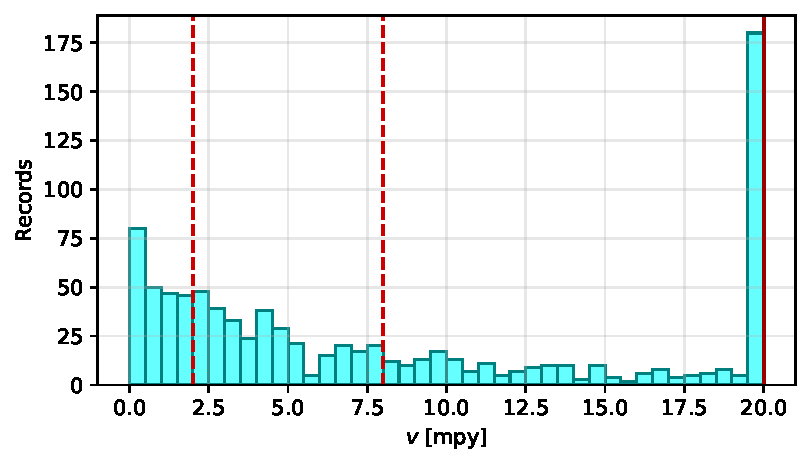
\includegraphics[width=0.9\linewidth]{figures/hist_target.pdf}
  \caption{Distribution of the measured corrosion rate after
    saturation. Dashed lines mark the normative limits at 2 [mpy] and
    8 [mpy]; the solid line marks the saturation level at 20 [mpy].}
  \label{fig:hist}
\end{figure}



  \section{Theoretical background}    \label{sec:theory} %================
    \subsection{Decision trees as rule generators}

A classification tree partitions the input space with axis-aligned thresholds and assigns one class to each terminal region \cite{breiman1984cart}. Each root-to-leaf path is a conjunction of interpretable conditions, so a trained tree is simultaneously a classifier and a rule generator. For imbalanced classes, accuracy rewards the majority class; the per-class recall (the fraction of each class recovered) and the recall ratio $\min(\mathrm{recalls})/\max(\mathrm{recalls})$ measure instead whether the classifier serves both classes. The acceptance criterion of this study requires a mean per-class recall above 0.6 with a balanced ratio, because an integrity classifier that misses the severe class is operationally useless regardless of its accuracy.

\subsection{Fuzzy inference with singleton consequents}

A fuzzy inference system evaluates a set of IF--THEN rules whose conditions hold to a degree between 0 and 1 given by membership functions \cite{zadeh1965fuzzy,mamdani1975experiment}. The firing strength of a rule is the minimum membership of its conditions. With singleton consequents $c_r$, the defuzzified output is the weighted average
\begin{equation}
  \hat{v}(\mathbf{x}) =
  \frac{\sum_{r} w_r(\mathbf{x})\, c_r}{\sum_{r} w_r(\mathbf{x})},
  \label{eq:fis}
\end{equation}
a Mamdani system with singleton output sets, equivalent to a zero-order Sugeno system \cite{takagi1985fuzzy}. The formulation produces a continuous output that interpolates smoothly between the rule consequents as the memberships shift, which is the property that converts a discrete severity classification into a numerical estimator.

\subsection{Nested cross-validation and leakage}
\label{sec:nested}

Model development involves selection: hyperparameters, thresholds, and design constants compete, and the winning combination is chosen because it scored best on some data. When the same data that guided the selection also produces the reported performance, the estimate is optimistically biased --- the selection has already ``seen'' the test labels, a form of information leakage \cite{varma2006bias,cawley2010overfitting}. Procedures that tune by cross-validation on the complete dataset and then refit on the same records suffer exactly this bias.

Nested cross-validation removes it with two loops (Figure~\ref{fig:nested}). The outer loop splits the data into five stratified folds; each outer test fold remains untouched during every selection and fitting step. Inside each outer training fold, an inner loop performs all the competitions: tree hyperparameters, leaf probability thresholds, and the transition-width factor of the membership functions. The complete chain then refits on the outer training fold and predicts the records of the outer test fold exactly once. The union of the five outer test folds yields out-of-fold predictions of every record, always produced by a model that never saw it. Metrics over this union estimate generalization to new monitoring points, because they reproduce the deployment situation: selection, fitting, and prediction never share records.

\begin{figure}[htb!]
  \centering
  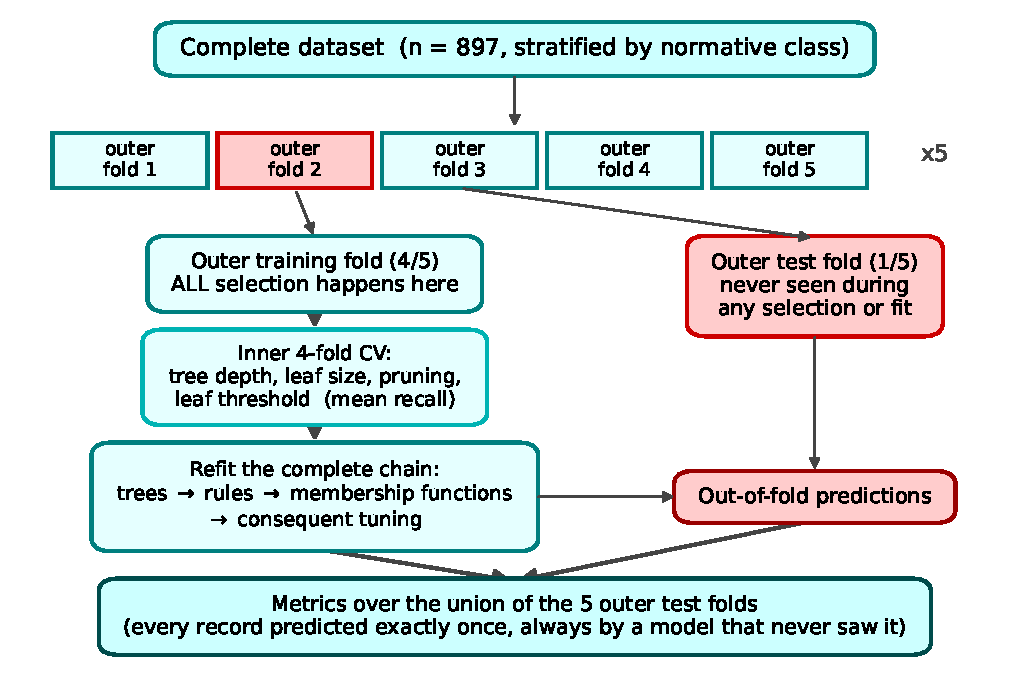
\includegraphics[width=\linewidth]{figures/nested_cv_scheme.pdf}
  \caption{Nested cross-validation protocol. Every selection step (inner 4-fold loop) and the complete refit of the chain occur inside the outer training fold; the outer test fold only receives predictions. The procedure repeats for the five outer folds, so every record is predicted exactly once by a model that never saw it.}
  \label{fig:nested}
\end{figure}

  \section{Methodology}               \label{sec:method} %================
    The strategy executes in four stages --- threshold-wise tree training,
rule extraction, membership-function construction, and consequent
tuning --- wrapped by the nested protocol of
Section~\ref{sec:nested}. Algorithm~\ref{alg:method} summarizes the
complete procedure.

\begin{algorithm}[htbp]
  \caption{Tree-rule fuzzy estimation of the corrosion rate}
  \label{alg:method}
  \KwIn{records $(\mathbf{x}_i, v_i)$, normative limits $L = \{2, 8\}$
    [mpy], saturation level $v_{\max} = 20$ [mpy]}
  \KwOut{fuzzy estimator $\hat{v}(\mathbf{x})$; out-of-fold metrics}
  saturate the target: $v_i \leftarrow \min(v_i, v_{\max})$\;
  \ForEach{outer fold $(\mathcal{T}, \mathcal{E})$ of the stratified
    5-fold split}{
    \tcp{all selection inside the training fold $\mathcal{T}$}
    select depth, leaf size, pruning and leaf threshold of each tree
    by inner CV maximizing mean recall\;
    fit binomial trees: $T_2$ for $v > 2$, $T_8$ for $v > 8$ on
    $\mathcal{T}$\;
    collapse sibling leaves of equal class; extract root-to-leaf
    paths as rules: $T_2^{-} \to$ low, $T_2^{+} \to$ mid,
    $T_8^{+} \to$ high\;
    merge near-duplicate thresholds; simplify each rule to one
    interval per variable\;
    select by inner CV (MAE) the numeric-layer configuration:
    rule-source trees (recall-selected or deeper variants),
    transition-width factor, and consequent regularization\;
    \ForEach{variable used by the rules}{
      partition its range at the tree thresholds\;
      build one interval membership per region: sigmoid shoulders
      crossing $0.5$ at the thresholds, width from the distance
      threshold--median of the training data, scaled by the selected
      factor\;
    }
    initialize each consequent $c_r$ at the median of its class;
    adjust all $c_r$ by regularized least squares on the normalized
    activations, bounded to the normative range of each rule\;
    predict $\mathcal{E}$ with Eq.~(\ref{eq:fis}), applying to the
    mid rules the ordinal exclusion
    $w \leftarrow \min(w,\, 1 - \max w_{\mathrm{high}})$\;
  }
  report metrics over the union of the outer test folds\;
  refit the complete chain on all records for deployment (artifacts
  only)\;
\end{algorithm}


\subsection{Binomial trees at the normative limits}

One binomial decision tree per normative limit provides the
classification backbone: $T_2$ answers whether the rate exceeds
2 [mpy] and $T_8$ whether it exceeds 8 [mpy]. Both use balanced class
weights. The hyperparameters --- depth (3--5), minimum leaf size
(3--10), cost-complexity pruning, and the leaf probability threshold
$\tau \in \{0.4, 0.5, 0.6\}$ --- compete in the inner folds under the
criterion mean recall $+\ 0.5 \times$ recall ratio, which targets the
acceptance condition of the application instead of accuracy.

\subsection{Rule extraction}

Each root-to-leaf path is a conjunction of threshold conditions.
Sibling leaves of the same class merge recursively, because their
split does not change the decision; the diagrams of the deployed trees
therefore match the rulebase one-to-one. The extraction assigns the
negative paths of $T_2$ to the consequent \emph{low}, the positive
paths of $T_2$ to \emph{mid}, and the positive paths of $T_8$ to
\emph{high}. Thresholds of one variable that differ by less than 1\%
of its robust range (1st--99th percentile) merge into one value, and
the conditions of each rule simplify to a single interval per
variable. Because the positive region of $T_2$ contains the severe
region, every \emph{mid} rule carries the ordinal exclusion \emph{AND
NOT (severe conditions)}, implemented as
$w \leftarrow \min(w, 1 - \max w_{\mathrm{high}})$.

\subsection{Interval membership functions}

For each variable used by the rulebase, its sorted tree thresholds
$t_1 < \dots < t_k$ partition the observed range into $k+1$ intervals,
and each interval defines one linguistic term. The term membership is
the minimum of two logistic shoulders: a rising shoulder anchored at
the lower threshold and a falling shoulder anchored at the upper
threshold. Each shoulder crosses 0.5 exactly at its threshold, which
preserves the correspondence between the tree partition and the fuzzy
partition. The transition width equals the distance from the threshold
to the median of the training data inside the interval, multiplied by
a scale factor selected in the inner folds
($s \in \{0.03, 0.1\}$); widths remain bounded by the robust span
of the variable so that outliers cannot distort the shape. A tree
condition $x \leq t_j$ maps to the maximum membership of the terms
left of $t_j$, and $x > t_j$ to the maximum of the terms right of it.

\subsection{Consequent tuning and inference}

Each rule receives a singleton consequent $c_r$ [mpy], initialized at
the median of the training records of its class and then adjusted by
box-constrained least squares on the normalized activation matrix:
$c_r$ must remain inside the normative range of its class (low:
$[0,2]$; mid: $[2,8]$; high: $[8, v_{\max}]$), with a regularization
$\lambda \in \{0.3, 1.0\}$, selected in the inner folds, that pulls
each consequent toward its class median. The constraint replaces the
manual support adjustment of classical fuzzy design with an auditable,
norm-consistent optimization: the expert reviews the tuned supports
knowing that no rule can speak outside its severity range. For the
numeric layer, the inner loop also chooses the rule-source trees among
the recall-selected ones and two deeper variants (depth 6--7): finer
partitions can carry additional regression signal, while the reported
classification always comes from the recall-selected trees. Inference
follows Eq.~(\ref{eq:fis}); when no rule fires, the system returns
the training median.

\subsection{Benchmarks}

Three regression methods suited to reduced databases compete on the
identical outer folds: linear regression, a decision-tree regressor
(depth 3--6, leaf size 3--10, selected in inner folds), and support
vector regression ($C \in \{1, 10, 100\}$,
$\epsilon \in \{0.1, 1.0\}$). Ensemble regressors with large parameter
counts remain outside the comparison because the reduced size of the
database raises their overfitting risk and their predictions do not
admit rule-level audit. Every benchmark uses median imputation and
standardization fitted inside the training folds.

  \section{Results and Discussion}    \label{sec:results} %===============
    \subsection{Classification at the normative limits}

Table~\ref{tab:trees} reports the out-of-fold metrics of the binomial trees. The 2 [mpy] tree reached a mean recall of 0.710 (0.646 for the non-exceeding class, 0.774 for the exceeding class) and the 8 [mpy] tree reached 0.808 with a recall ratio of 0.986. Both trees exceed the acceptance threshold of 0.6 with balanced per-class sensitivity. Figure~\ref{fig:cm} shows the three-class confusion matrix composed from the two out-of-fold binary decisions: the strategy recovers 0.60, 0.47, and 0.75 of the low, medium, and high classes, with the adjacent medium class as the hardest region.

\begin{table}[htb!]
\centering
\footnotesize
\setlength{\tabcolsep}{4pt}
\caption{Binomial decision trees at the normative limits: out-of-fold metrics of the nested cross-validation (Mean: mean per-class recall; Ratio: min/max recall).}
\label{tab:trees}
\begin{tabular}{@{}cccccc@{}}
\toprule
Limit & Mean & Ratio & Recall$_{\leq}$ & Recall$_{>}$ & Acc. \\
\midrule
\midrule
2 [mpy] & 0.710 & 0.834 & 0.646 & 0.774 & 0.742 \\
8 [mpy] & 0.808 & 0.986 & 0.803 & 0.814 & 0.807 \\
\bottomrule
\end{tabular}
\end{table}


\begin{figure}[htb!]
  \centering
  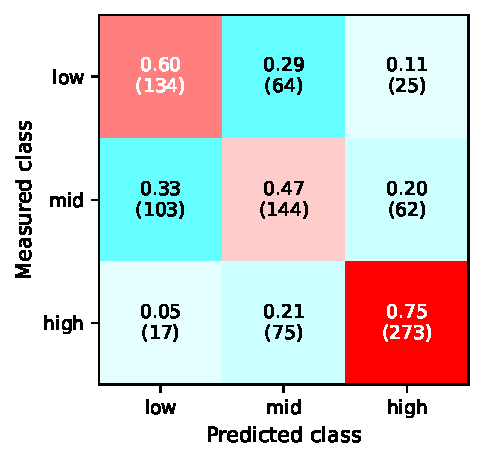
\includegraphics[width=0.62\linewidth]{figures/confusion_matrix.pdf}
  \caption{Three-class out-of-fold confusion matrix (row-normalized; record counts in parentheses).}
  \label{fig:cm}
\end{figure}

Figure~\ref{fig:trees} presents the deployed trees. Both organize the fleet by its service history and geometry: the 2 [mpy] tree separates the monitoring regime by service time, flow velocity, and gas rate, and the 8 [mpy] tree isolates the severe regime among the young, small-diameter, gas-rich lines.

\begin{figure*}[htb!]
  \centering
  \begin{subfigure}{0.85\textwidth}
    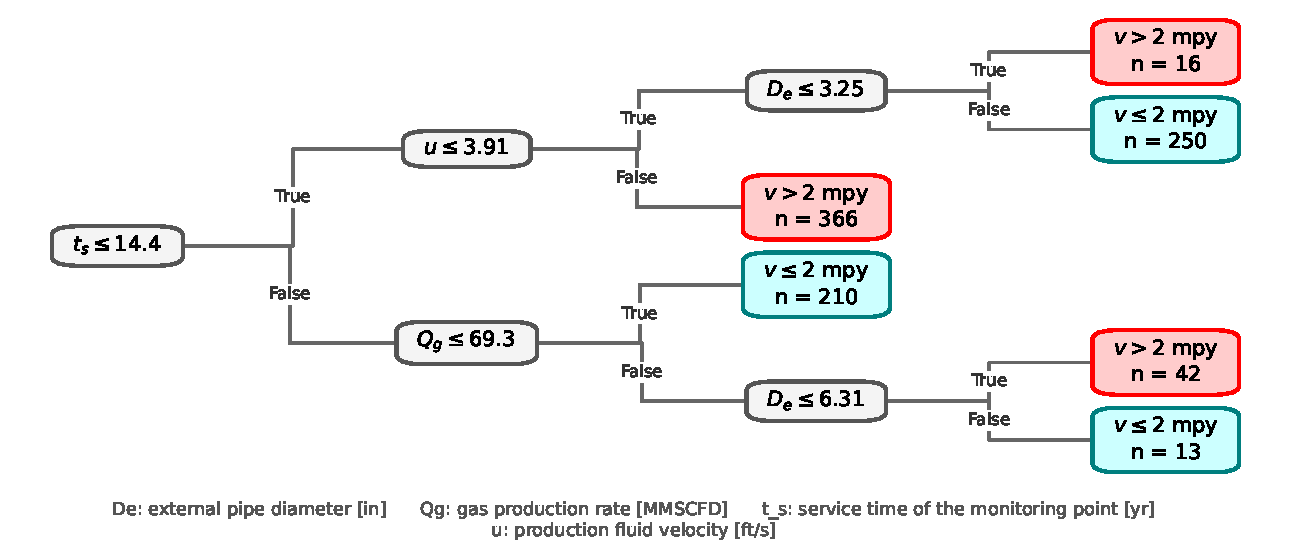
\includegraphics[width=\linewidth]{figures/tree_th2.pdf}
    \caption{}
  \end{subfigure}
  \begin{subfigure}{0.95\textwidth}
    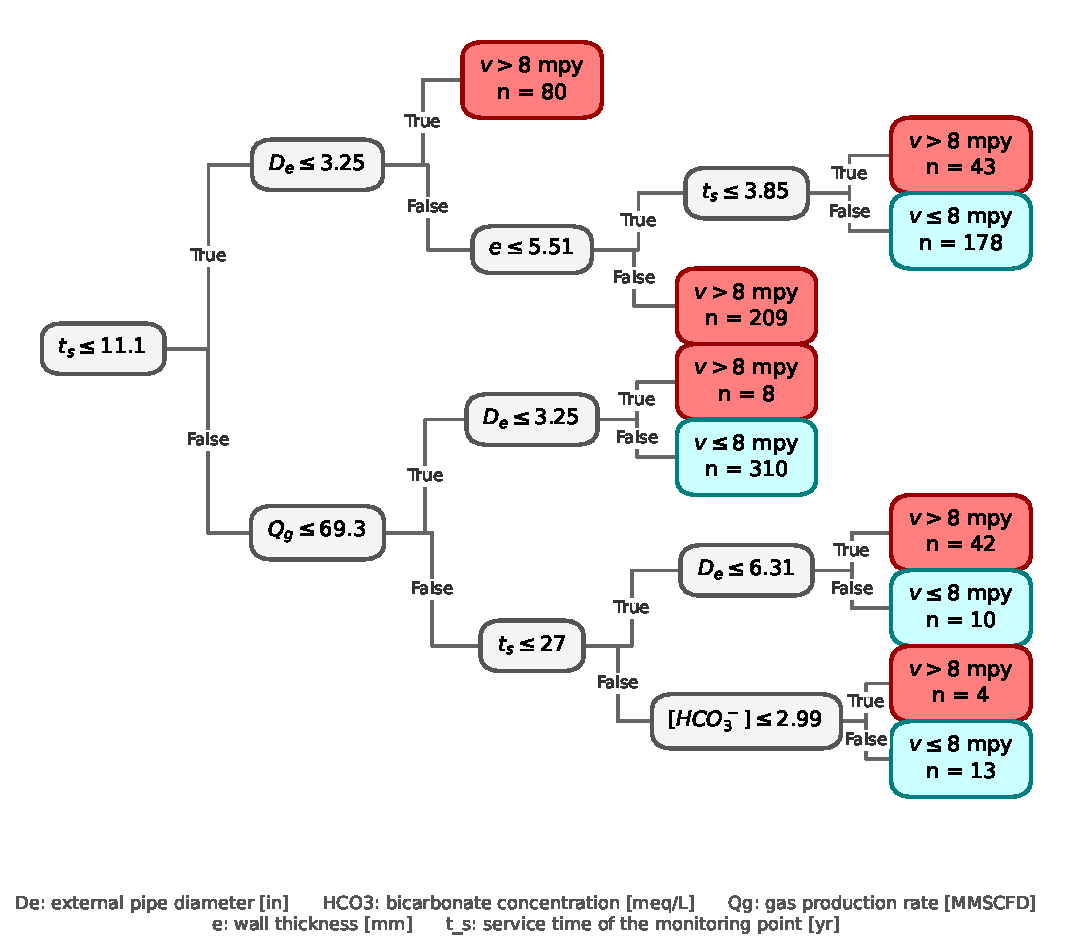
\includegraphics[width=\linewidth]{figures/tree_th8.pdf}
    \caption{}
  \end{subfigure}
  \caption{Deployed binomial trees after merging the partitions that do not change the decision: (a) 2 [mpy] limit, (b) 8 [mpy] limit. Teal leaves do not exceed the limit; red leaves exceed it; $n$ is the number of training records per leaf.}
  \label{fig:trees}
\end{figure*}

\subsection{Deployed rulebase and physical reading}

The full-data refit produced twelve rules over six variables: the service time $t_s$, the fluid velocity $u$, the external diameter $D_e$, the gas rate $Q_g$, the wall thickness $e$, and the bicarbonate concentration $[\mathrm{HCO_3^-}]$ (Table~\ref{tab:rules}). Figure~\ref{fig:coverage} quantifies the share of the output that each rule carries within its own severity zone. The rules organize the asset population by its service history and duty:

\begin{itemize}
  \item \textbf{R1} (low, $c_1 = 2.0$ [mpy]): young lines ($t_s \leq 14$ [yr]) of larger diameter ($D_e > 3.25$ [in]) under slow flow ($u \leq 3.9$ [ft/s]): low wall shear on a large section keeps the attack inside the monitoring range.
  \item \textbf{R2} (low, $c_2 = 1.2$ [mpy]): mature lines ($t_s > 14$ [yr]) with low gas rate ($Q_g \leq 69$ [MMSCFD]). This is the dominant low rule (46\% of the zone): a line that has survived beyond fourteen years under quiet service demonstrates a benign environment, and the low gas rate limits turbulence and CO$_2$ supply.
  \item \textbf{R3} (low, $c_3 = 2.0$): mature lines with high gas rate but large diameter ($D_e > 6.3$ [in]): the section area keeps the mixture velocity, and with it the wall shear, low.
  \item \textbf{R4} (mid, $c_4 = 7.1$): young, slow, small-diameter lines. The ordinal exclusion suppresses this rule completely (0\% contribution): its region belongs to the severe rule R7, which demonstrates the exclusion operating as designed.
  \item \textbf{R5} (mid, $c_5 = 6.0$): young lines under fast flow ($u > 3.9$ [ft/s]): flow-enhanced attack before any protective layer consolidates. Dominant medium rule (22\% of the zone).
  \item \textbf{R6} (mid, $c_6 = 6.2$): mature, gas-rich lines of small diameter: the sustained turbulence keeps the rate in the intensified-inspection range.
  \item \textbf{R7} (high, $c_7 = 19.9$): young, small-diameter lines ($t_s \leq 11$ [yr], $D_e \leq 3.25$ [in]): the highest-severity population of the fleet. Small sections concentrate velocity and wall shear, and the early failures of the field concentrate here (21\% of the severe zone).
  \item \textbf{R8, R9} (high, $c_8 = 16.7$, $c_9 = 14.5$): young larger-diameter lines, separated by wall thickness ($e$ at 5.5 [mm]); R9 is the dominant severe rule (35\% of the zone). Youth with damage already visible marks aggressive service across design classes.
  \item \textbf{R10} (high, $c_{10} = 19.7$): mature small-diameter lines under low gas rate that still exceed 8 [mpy]: a residual severe population where geometry dominates.
  \item \textbf{R11} (high, $c_{11} = 12.4$): intermediate-age lines ($11 < t_s \leq 27$ [yr]) with high gas rate: sustained turbulent duty keeps mature lines in the severe range.
  \item \textbf{R12} (high, $c_{12} = 9.7$): old gas-rich lines with depleted bicarbonate ($[\mathrm{HCO_3^-}] \leq 3$ [meq/L]): without carbonate buffering no protective scale forms, and even old lines remain above the intervention limit.
\end{itemize}

The service time carries a double meaning in this reading. It is a legitimate covariate --- fixed at installation and known before any measurement --- and the audit of Section~\ref{sec:vmod} explains why young lines concentrate the high reported rates: the reported rate averages the accumulated loss over the service time for most records, so equal damage produces higher rates on younger lines. The rulebase therefore ranks the current severity of the fleet, with young, small-diameter, gas-rich lines at the top --- exactly the population that the integrity program inspects first.

\begin{table}[htb!]
\centering
\footnotesize
%\setlength{\tabcolsep}{4pt}
\caption{Deployed rulebase: antecedents extracted from the binomial trees (physics nomenclature), tuned consequent singletons $c_r$ and contribution share of each rule to the output within its own severity zone.}
\label{tab:rules}
\begin{tabularx}{0.45\textwidth}{@{}lXrr@{}}
\toprule
Rule & Antecedent & $c_r$ [mpy] & Contrib. [\%] \\
\midrule
\midrule
\multicolumn{4}{@{}l}{\emph{Consequent: low}} \\
R1 & $t_s \leq 14.4 \wedge u \leq 3.91 \wedge D_e > 3.25$ & 2.00 & 24.3 \\
R2 & $t_s > 14.4 \wedge Q_g \leq 69.3$ & 1.22 & 46.1 \\
R3 & $t_s > 14.4 \wedge Q_g > 69.3 \wedge D_e > 6.31$ & 2.00 & 4.9 \\
\midrule
\multicolumn{4}{@{}l}{\emph{Consequent: mid }} \\ %(each rule also carries the exclusion $\neg S$ of the severe region)
R4 & $t_s \leq 14.4 \wedge u \leq 3.91 \wedge D_e \leq 3.25$ & 7.09 & 0.0 \\
R5 & $t_s \leq 14.4 \wedge u > 3.91$ & 6.03 & 22.4 \\
R6 & $t_s > 14.4 \wedge Q_g > 69.3 \wedge D_e \leq 6.31$ & 6.19 & 3.9 \\
\midrule
\multicolumn{4}{@{}l}{\emph{Consequent: high}} \\
R7 & $t_s \leq 11.1 \wedge D_e \leq 3.25$ & 19.90 & 21.5 \\
R8 & $t_s \leq 3.85 \wedge D_e > 3.25 \wedge e \leq 5.51$ & 16.71 & 7.4 \\
R9 & $t_s \leq 11.1 \wedge D_e > 3.25 \wedge e > 5.51$ & 14.51 & 34.6 \\
R10 & $t_s > 11.1 \wedge Q_g \leq 69.3 \wedge D_e \leq 3.25$ & 19.65 & 1.7 \\
R11 & $t_s > 11.1 \wedge t_s \leq 27 \wedge Q_g > 69.3 \wedge D_e \leq 6.31$ & 12.38 & 10.8 \\
R12 & $t_s > 27 \wedge Q_g > 69.3 \wedge [\mathrm{HCO_3^-}] \leq 2.99$ & 9.74 & 0.6 \\
\bottomrule
\end{tabularx}
\end{table}


\begin{figure}[htb!]
  \centering
  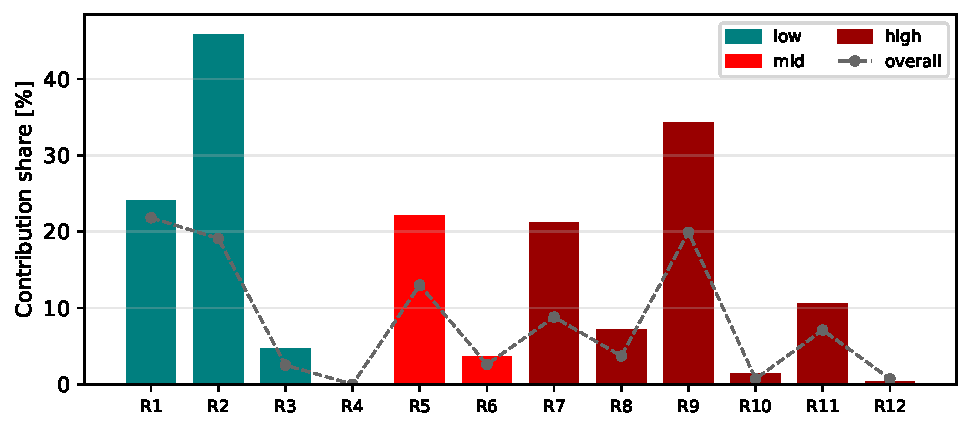
\includegraphics[width=\linewidth]{figures/rule_coverage.pdf}
  \caption{Contribution share of each rule to the fuzzy output: bars, within the records of the rule's own severity zone; dashed line, over all records. Colors follow the severity of the consequent.}
  \label{fig:coverage}
\end{figure}

\subsection{Membership functions and consequents}

Figure~\ref{fig:mfs} shows the interval membership functions of the two variables that appear most often in the rulebase and the linguistic partition of the output. Every transition crosses 0.5 exactly at a tree threshold, so the fuzzy partition remains traceable to the trees; the transition widths follow the training-data distribution inside each interval, with the sharpness factor selected in the inner folds. Figure~\ref{fig:singletons} presents the tuned consequent singletons: the least-squares adjustment spreads them inside their normative ranges without violating any boundary, and the six severe consequents grade the intervention range from 9.7 to 19.9 [mpy].

\begin{figure*}[htb!]
  \centering
  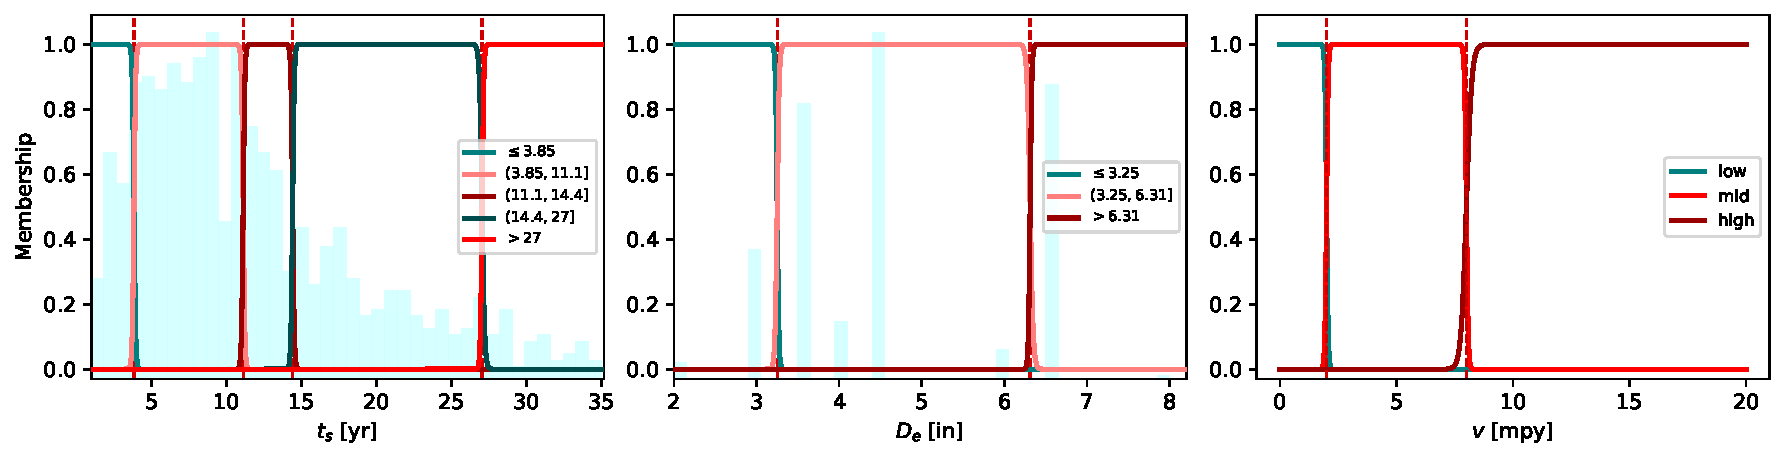
\includegraphics[width=\textwidth]{figures/mf_three_panel.pdf}
  \caption{Interval membership functions derived from the tree thresholds (dashed lines): (a) service time $t_s$, (b) external diameter $D_e$, with the training histograms in the background; (c) linguistic partition of the output variable at the normative limits.}
  \label{fig:mfs}
\end{figure*}

\begin{figure}[htb!]
  \centering
  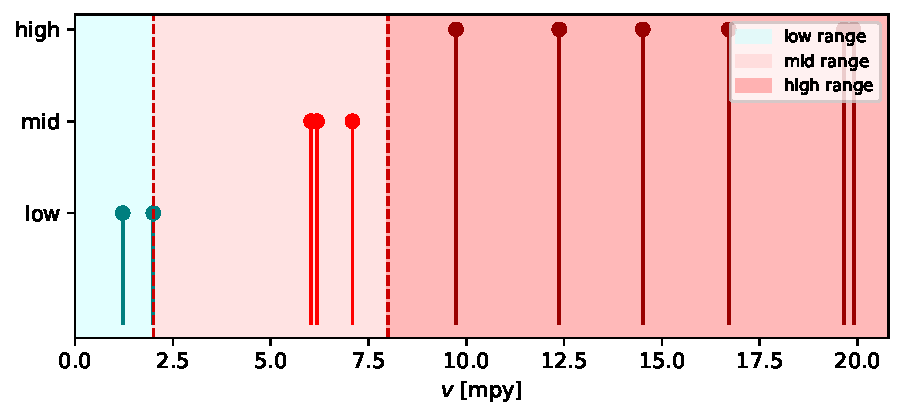
\includegraphics[width=\linewidth]{figures/consequent_singletons.pdf}
  \caption{Tuned consequent singletons of the twelve rules within the normative ranges (shaded). Dashed lines mark the 2 [mpy] and 8 [mpy] limits.}
  \label{fig:singletons}
\end{figure}

\subsection{Predictive performance}

The out-of-fold parity of the fuzzy system: an $R^2$ of 0.50, an MAE of 3.65 [mpy], and an RMSE of 5.20 [mpy] over the 897 records. Figure~\ref{fig:response} demonstrates the property promised by the formulation: sweeping the service time with the remaining variables at their medians produces a continuous output that ramps across the normative limits instead of jumping between class labels.

\begin{figure}[htb!]
  \centering
  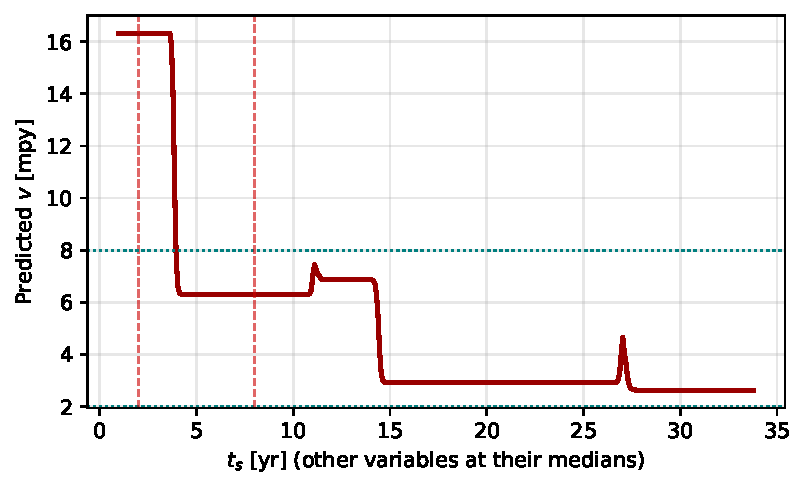
\includegraphics[width=0.9\linewidth]{figures/response_curve.pdf}
  \caption{Response of the fuzzy system to the service time with the remaining variables at their medians. The output ramps smoothly across the normative limits (dashed and dotted lines).}
  \label{fig:response}
\end{figure}

\subsection{Comparison on identical folds}

Table~\ref{tab:comparison} and Figure~\ref{fig:box} compare the four methods under the identical nested protocol, reporting the global out-of-fold value and the minimum--maximum band across the five outer folds. The fuzzy system reaches the lowest MAE after the decision-tree regressor (3.65 against 3.34 [mpy]) and surpasses linear regression (4.15 [mpy]) and support vector regression (3.82 [mpy]); its $R^2$ of 0.498 exceeds both (0.492 and 0.486) and remains within 0.04 units of the decision-tree regressor (0.540).

\begin{table}[htb!]
\centering
\footnotesize
\setlength{\tabcolsep}{4pt}
\caption{Out-of-fold comparison on identical folds: global value (min--max across the five outer folds).}
\label{tab:comparison}
\begin{tabular}{@{}lccc@{}}
\toprule
Method & MAE [mpy] & $R^2$ & Recall$_{high}$ \\
\midrule
\midrule
Proposed FIS & 3.65 (3.22--4.21) & 0.498 (0.38--0.60) & 0.78 \\
Linear reg. & 4.15 (3.87--4.47) & 0.492 (0.44--0.54) & 0.89 \\
Decision-tree reg. & 3.34 (2.99--3.79) & 0.540 (0.47--0.58) & 0.78 \\
SVR & 3.82 (3.43--4.26) & 0.486 (0.42--0.54) & 0.80 \\
\bottomrule
\end{tabular}
\end{table}


\begin{figure*}[htb!]
  \centering
  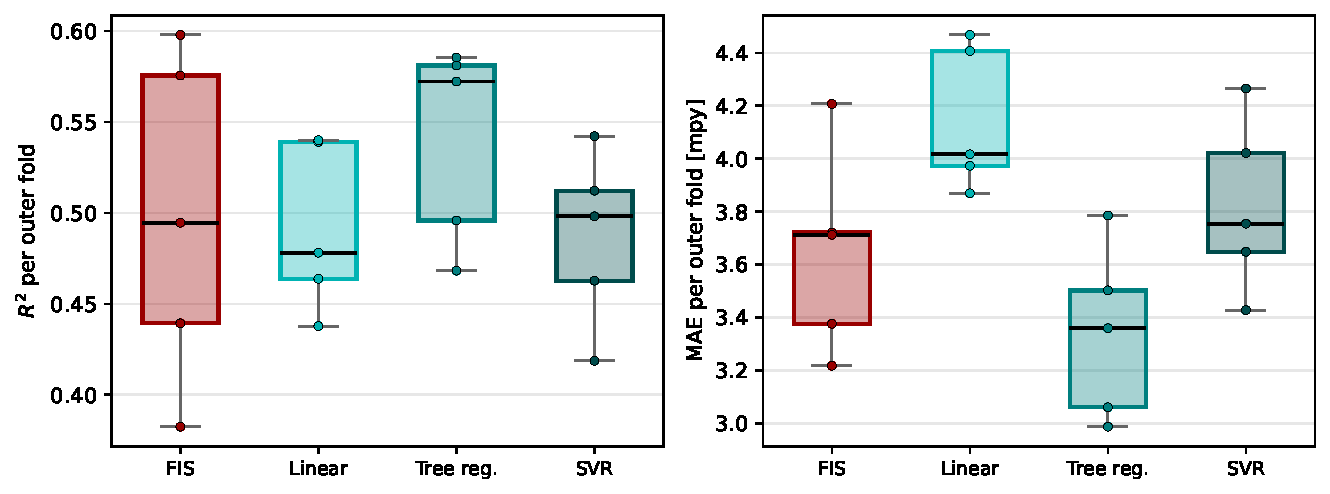
\includegraphics[width=0.92\textwidth]{figures/nested_boxplots.pdf}
  \caption{Per-fold distribution of $R^2$ and MAE for the four methods under the identical nested protocol (five outer folds; boxes span the interquartile range, whiskers the full min--max band, points mark the individual folds).}
  \label{fig:box}
\end{figure*}

Figure~\ref{fig:zones} decomposes the error by severity zone. The fuzzy system improves on linear regression in every zone (3.14 against 4.02 [mpy] in the low zone, 2.82 against 3.30 in the medium zone, and 4.66 against 4.94 in the high zone) and attains the lowest low-zone error of all four methods. Thresholding the continuous outputs at the normative limits shows why the strategy separates the classification and estimation roles: thresholded linear regression recovers the high class strongly (recall 0.89) only by overpredicting --- its low-class recall collapses to 0.31 --- whereas the dedicated classification layer of the strategy delivers balanced recalls (0.80 and 0.81 at the 8 [mpy] limit).

\begin{figure}[htb!]
  \centering
  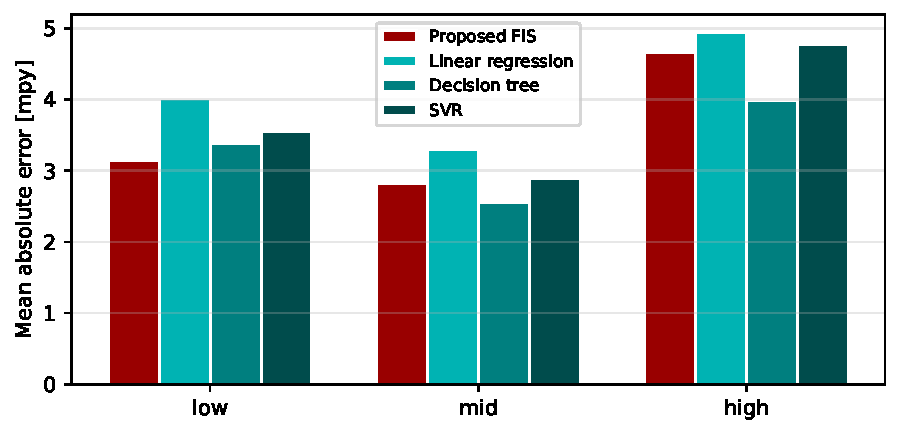
\includegraphics[width=\linewidth]{figures/error_by_zone.pdf}
  \caption{Mean absolute out-of-fold error by severity zone for the
    four methods.}
  \label{fig:zones}
\end{figure}

\subsection{Why the decision-tree regressor is less interpretable}

The decision-tree regressor offers the lowest global error, and a single tree is often presented as an interpretable model. Four structural facts separate it from the proposed system in this application.

First, its complexity: the trees selected by the inner loops carry between 15 and 45 leaves per fold. Each leaf is one disjoint rule, so the regressor speaks through 15--45 rules, against twelve rules with at most four conditions. An expert can audit twelve propositions; a forty-leaf partition exceeds the practical limit of rule-by-rule verification.

Second, its consequents: each leaf outputs the unconstrained mean of its training records. Nothing ties these constants to the normative classes --- a leaf mean can sit anywhere, and no boundary separates a ``monitoring'' leaf from an ``intervention'' leaf. The proposed system bounds every consequent to the normative range of its severity class, so each rule speaks the language of the standard.

Third, its output geometry: the prediction is piecewise constant. The estimate jumps discontinuously when a variable crosses a threshold and remains flat elsewhere, which contradicts the gradual character of the corrosion phenomenon. The fuzzy system produces the smooth, monotone transitions of Figure~\ref{fig:response}.

Fourth, its severity structure: the regressor optimizes a global error without any notion of the normative classes, and its induced classification is as unbalanced as that of the other regressors. The proposed strategy carries a dedicated classification layer designed for exactly that criterion.

The comparison therefore delimits the position of each method: the fuzzy system concedes 0.04 units of $R^2$ in exchange for a continuous output with smooth transitions, consequents bounded to the normative ranges, a balanced severity classification, and a twelve-rule inference chain in which every prediction traces to explicit, verifiable service and operating conditions.

  \section{Conclusions}               \label{sec:conclu} %================
    This study developed and validated a strategy that converts binomial decision trees at the normative severity limits into an auditable fuzzy estimator of the corrosion rate for reduced, imbalanced field databases.

The classification layer satisfied the normative acceptance condition under a nested cross-validation protocol that confines every selection step to inner folds: out-of-fold mean per-class recalls of 0.710 at the 2 [mpy] limit and 0.808 at the 8 [mpy] limit, with recall ratios of 0.83 and 0.99, on the internal-corrosion database of 897 records. The trees organize the fleet by its service time, geometry, and gas duty, and isolate the severe regime among the young, small-diameter, gas-rich lines.

The fuzzy layer converted the twelve extracted rules into a continuous estimator through interval membership functions anchored at the tree thresholds and consequent singletons bounded to the normative ranges. The system reached an out-of-fold $R^2$ of 0.50 and an MAE of 3.65 [mpy], surpassing linear regression ($R^2 = 0.49$, MAE = 4.15 [mpy]) and support vector regression on identical folds, with a lower error than linear regression in every severity zone. Against the decision-tree regressor, which attains a lower global error with 15--45 unconstrained leaves, the fuzzy system concedes 0.04 units of $R^2$ in exchange for a smoother output, normative-bounded consequents, and a twelve-rule inference chain whose every proposition admits verification against the service history of the asset.

The strategy therefore delivers the property that motivated it: a numerical corrosion-rate estimator whose complete inference chain --- rule, membership, and bounded consequent --- admits expert audit, built on the knowledge already contained in the inspection program and the operating data. Future work will extend validation to additional asset families, incorporate expert revisions of individual thresholds into the deployment cycle, and enrich the databases with variables measured independently of the inspection that defines the target.

    \bibliography{references}

\end{document}
